\documentclass[]{article}
\usepackage{amsmath}
\usepackage{amssymb}
\usepackage{amsthm}
\usepackage{listings}
\usepackage{multirow}
\usepackage{tikz}
\usepackage{tikz-qtree}
\usepackage{tipa}
\usetikzlibrary{arrows,automata}
\begin{document}
\newcommand*{\xml}[1]{\texttt{<#1>}}
\theoremstyle{definition}
\newtheorem{thm}{Theorem}

\title{COMS W3261 \\ Computer Science Theory \\ Lecture 11\\ Closure and 
Decision Properties of CFL's}
\author{Alexander Roth}
\date{2014 -- 10 -- 08}
\maketitle

\section*{Outline}
  \begin{enumerate}
    \item Closure properties of CFL's
    \item Nonclosure properties of CFL's
    \item Cocke-Younger-Kasami algorithm
    \item Testing emptiness of a CFG
    \item Undecidable CFL problems
  \end{enumerate}
  
\section{Closure Properties of CFL's}
  \begin{itemize}
    \item The context-free languages are closed under the following operations:
      \begin{itemize}
        \item Substitution
          \begin{itemize}
            \item Let $\Sigma$ be an alphabet and let $L_a$ be a language for 
            each symbol $a$ in $\Sigma$. These languages define a substitution 
            $s$ on $\Sigma$.
            \item If $w = a_1a_2\ldots{}a_n$ is a string in $\Sigma^*$, then
            $s(w) = \{ x_1x_2\ldots{}x_n \, | \, x_i$ is a string in $s(a_i)$ 
            for $1 \leq i \leq n \}$.
            \item If $L$ is a language, $s(L) = \{s(w)\,|\,w$ is in $L \}$.
            \item If $L$ is a CFL over $\Sigma$ and $s(a)$ is a CFL for each 
            $a$ in $\Sigma$, then $s(L)$ is a CFL.
          \end{itemize}
        \item Union
        \item Concatenation
        \item Kleene star
        \item Homomorphism
        \item Reversal
        \item Intersection with a regular set
        \item Inverse Homomorphism
      \end{itemize}
  \end{itemize}
  
\section{Nonclosure Properties of CFL's}
  \begin{itemize}
    \item The context-free languages are not closed under the following operations:
      \begin{itemize}
        \item Intersection
          \begin{itemize}
            \item $L_1 = \{ a^nb^nc^i \, | \,n, i \leq 0 \}$ and 
            $L_2 = \{ a^ib^nc^n \, | \, n, i \leq 0 \}$ are CFL's. But
            $L = L_1 \cap L_2 = \{a^nb^nc^n \, | \, n \geq 0 \}$ is not a CFL.
          \end{itemize}
        \item Complement
          \begin{itemize}
            \item Suppose $comp(L)$ is context free if $L$ is context free. 
            Since $L_1 \cap L_2 = comp(comp(L_1) \cup comp(L_2))$, this would
            imply the CFL's are closed under intersection.
          \end{itemize}
        \item Difference
          \begin{itemize}
            \item Suppose $L_1 - L_2$ is context free if $L_1$ and $L_2$ are 
            context free. If $L$ is a CFL over $\Sigma$, then 
            $comp(L) = \Sigma^* - L$ would be context free.
          \end{itemize}
      \end{itemize}
  \end{itemize}
  
\section{Cocke-Younger-Kasami Algorithm for Testing Membership in a CFL}
  \begin{itemize}
    \item Input: a Chomsky normal form CFG $G = (V,T,P,S)$ and a string $w = 
    a_1a_2\ldots{a_n}$ in $T^*$.
    \item Output: ``yes'' if $w$ is in $L(G)$, ``no'' otherwise.
    \item Method: The CYK algorithm is a dynamic programming algorithm that 
    fils in a triangular table $x_{ij}$ with nonterminals $A$ such that $A 
    \overset{*}{\Rightarrow} a_ia_i+j\ldots{a_j}$.
      \begin{figure}[p]
        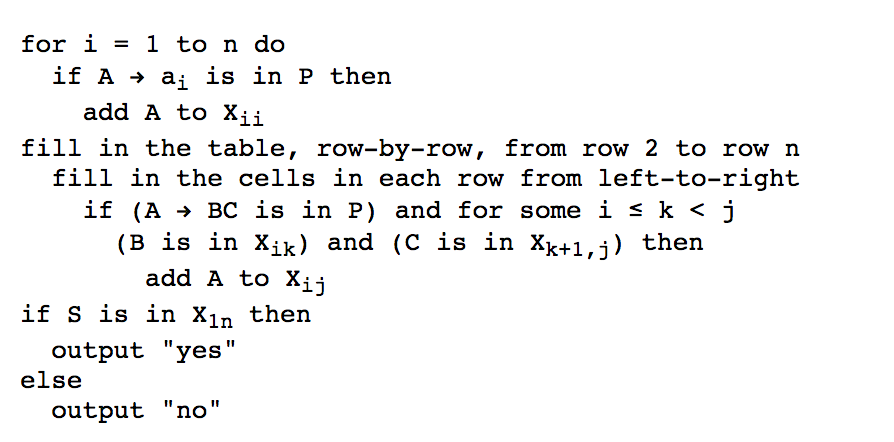
\includegraphics{./img/CYK_Algorithm.png}
        \caption{The CYK Algorithm in Pseudocode}
      \end{figure}
    \item The algorithm adds nonterminal $A$ to $x_{ij}$ iff there is a 
    production $A \rightarrow BC$ in $P$ where $B \overset{*}{\Rightarrow}
    a_ia_{i+1}\ldots{a_k}$ and $C \overset{*}{\Rightarrow}a_{k+1}a_{k
    +2}\ldots{a_j}$.
    \item To compute entry $x_{ij}$, we examine at most $n$ pairs of entries: 
    $(x_{ii},x_{i+1},_j)$,$(x_i,_{i+1},x_{i+2},_j)$, and so on until $
    (x_i,_{j-1},x_{j},_j)$.
    \item The running time of the CYK algorithm is $O(n^3)$.
  \end{itemize}

\section{Testing Emptiness of a CFG}
  \begin{itemize}
    \item Problem: Given a CFG $G$, is $L(G)$ empty?
    \item Emptiness problem is decidable: determine whether the start symbol of
    $G$ is generating.
      \begin{itemize}
        \item Naive algorithm has $O(n^2)$ time complexity where $n$ is the 
        size of $G$ (sum of the lengths of the productions).
        \item With a more sophisticated list-processing algorithm, emptiness 
        problems can be solved in linear time. See HMU, p. 302.
      \end{itemize}
  \end{itemize}
  
\section{Undecidable CFL Problems}
  \begin{itemize}
    \item We say a problem that cannot be solved by any Turing machine is
    \emph{undecidable}. There is no algorithm that can solve an undecidable
    problem.
    \item We shall see that several fundamental questions about context-free
    grammars and languages are undecidable, such as:
      \begin{enumerate}
        \item Is a given CFG ambiguous?
        \item Given a CFG, is there another equivalent CFG that is 
        unambiguous?
        \item Do two given CFG's generate the same language?
        \item Is the intersection of the languages generated by two CFG's 
        empty?
        \item Given a CFG $G = (V,T,P,s)$, is $L(G) = T^*$?
      \end{enumerate}
  \end{itemize}

\end{document}